\section{\uppercase{Discussion and Limitations}}
\label{sec:discussion}
\noindent Correct computation and exact binding cannot ensure selection of the requested result. Case~15 contains personal insufficiency but substitutes valid earlier comparisons for the requested recent-peer answer. Silently inserting that answer would hide the selection failure being studied.\draftassist

\begin{figure*}[!t]
\centering
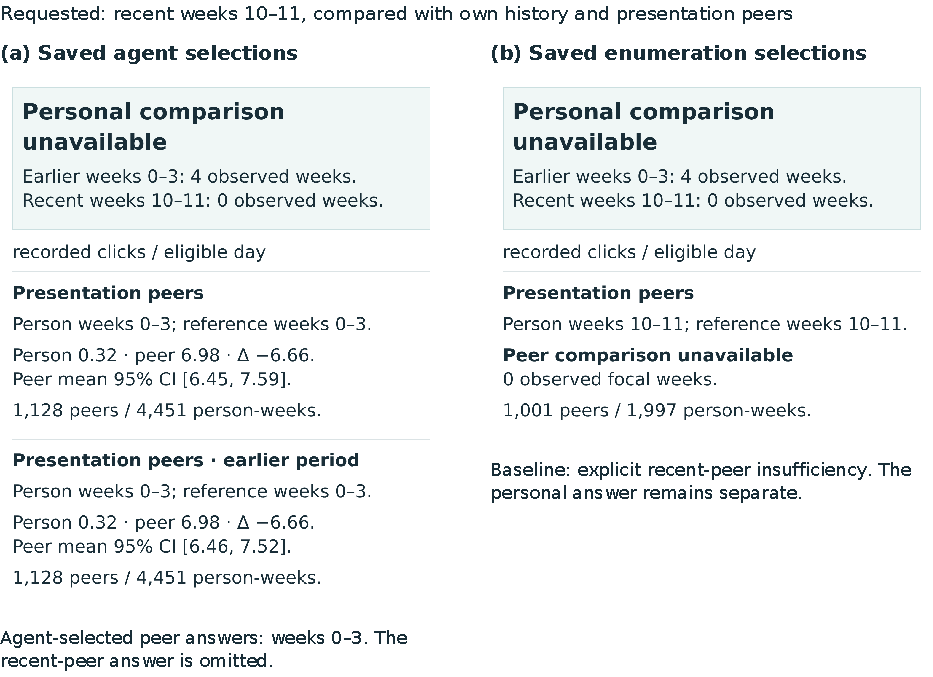
\includegraphics[width=\textwidth]{figures/failure.pdf}
\caption{Correct source-bound values with an incomplete answer, case~15. The request concerns weeks~10--11 and separately asks about own history and peers. (a) A selects earlier peer answers for weeks~0--3 and retains a personal-insufficiency answer. (b) Enumeration explicitly supplies the recent-peer insufficiency answer, also retaining personal insufficiency. Reviewer annotations outside the faithful excerpts identify the mismatch; the agent's missing answer is not inserted. Full original dashboards, not these cropped views, determine the frozen judgment. Intervals describe peer means; unavailable is not zero.}
\label{fig:failure}
\end{figure*}

\subsection{What the Ablation Establishes}
Explicit identity yielded no frozen visible gain over B and lower completeness than A. B's higher acceptance did not establish better coverage, and its catalogue prevents attributing effects solely to metadata derivation. Traces expose selection relevance, malformed requests, and incomplete scope coverage without isolating their causal contributions.

Counting all visible context as agent reasoning would overstate model responsibility; treating every frozen omission as literal absence would misdescribe B17--20. Provenance and equivalent-answer adjudication are both needed. Additional panels alone do not establish a better answer.

Enumeration remains the operational baseline. Its public task-family label and small registry make exhaustive rules feasible; success does not establish unrestricted language understanding. Agent benefits for ambiguous requests, larger registries, or other domains remain untested. Neither a per-case best-condition mixture nor further indefinite prompt tuning is justified.

\subsection{Presentation as an Inspectable System Behavior}
Figure~\ref{fig:reference} holds the focal rate at 3.50 clicks per eligible day while switching recent/earlier peer means of 3.46/6.98. Saved differences are +0.04/$-3.48$, calculated before rounding. Changed period and membership remain visible. This shows reference dependence of a description, not causation or reference superiority.

The assessment view foregrounds measures and events. In A17, recent weeks~8--11 have 0.25 non-banked submissions per observed week and zero scheduled non-submissions, while a day-55 snapshot records no submission for the day-54 assessment. Their temporal scopes differ; later submissions do not rewrite earlier snapshots. Grades and banking approval remain unavailable, not achievement ratings. This is implemented adaptation, not measured usability or accuracy improvement.

\subsection{Threats to Interpretation}
There are 24 development people from two offerings, not 96 independent observations. Families and wording conventions were known. One checkpoint, greedy episode, and environment do not establish robustness across models, paraphrases, runs, or deployments. Reserved people remain unevaluated; earlier development is not independent confirmation.

The rubric needs adjudication against question meaning. Numerical agreement cannot settle reference appropriateness, support thresholds, or equivalent answers. Independent forms for all 96 slots remain blank; human review and usability evaluation are pending.

Repeated rows, unknown logging and grade timing, eligibility, changing peers, and unequal histories limit measurement interpretation. Bootstrap intervals do not quantify measurement error, causality, or individual risk. No prediction, anomaly detection, or assessment of ability is validated. Presentation does not remedy these limits.

Any adjudicated reanalysis must be separately versioned as post hoc. Stronger reliability claims need a fixed system/scorer, person-level sampling, enumeration controls, and prespecified outcomes before reserved-data evaluation. The internal gate is not a conference acceptance requirement; its failure limits operational claims, rather than automatically invalidating a negative development study.
